\documentclass{standalone}
\usepackage{tikz}
\usetikzlibrary{patterns, positioning}
\usepackage[sfdefault]{ClearSans} %% option 'sfdefault' activates Clear Sans as the default text font
\usepackage[T1]{fontenc}

\begin{document}
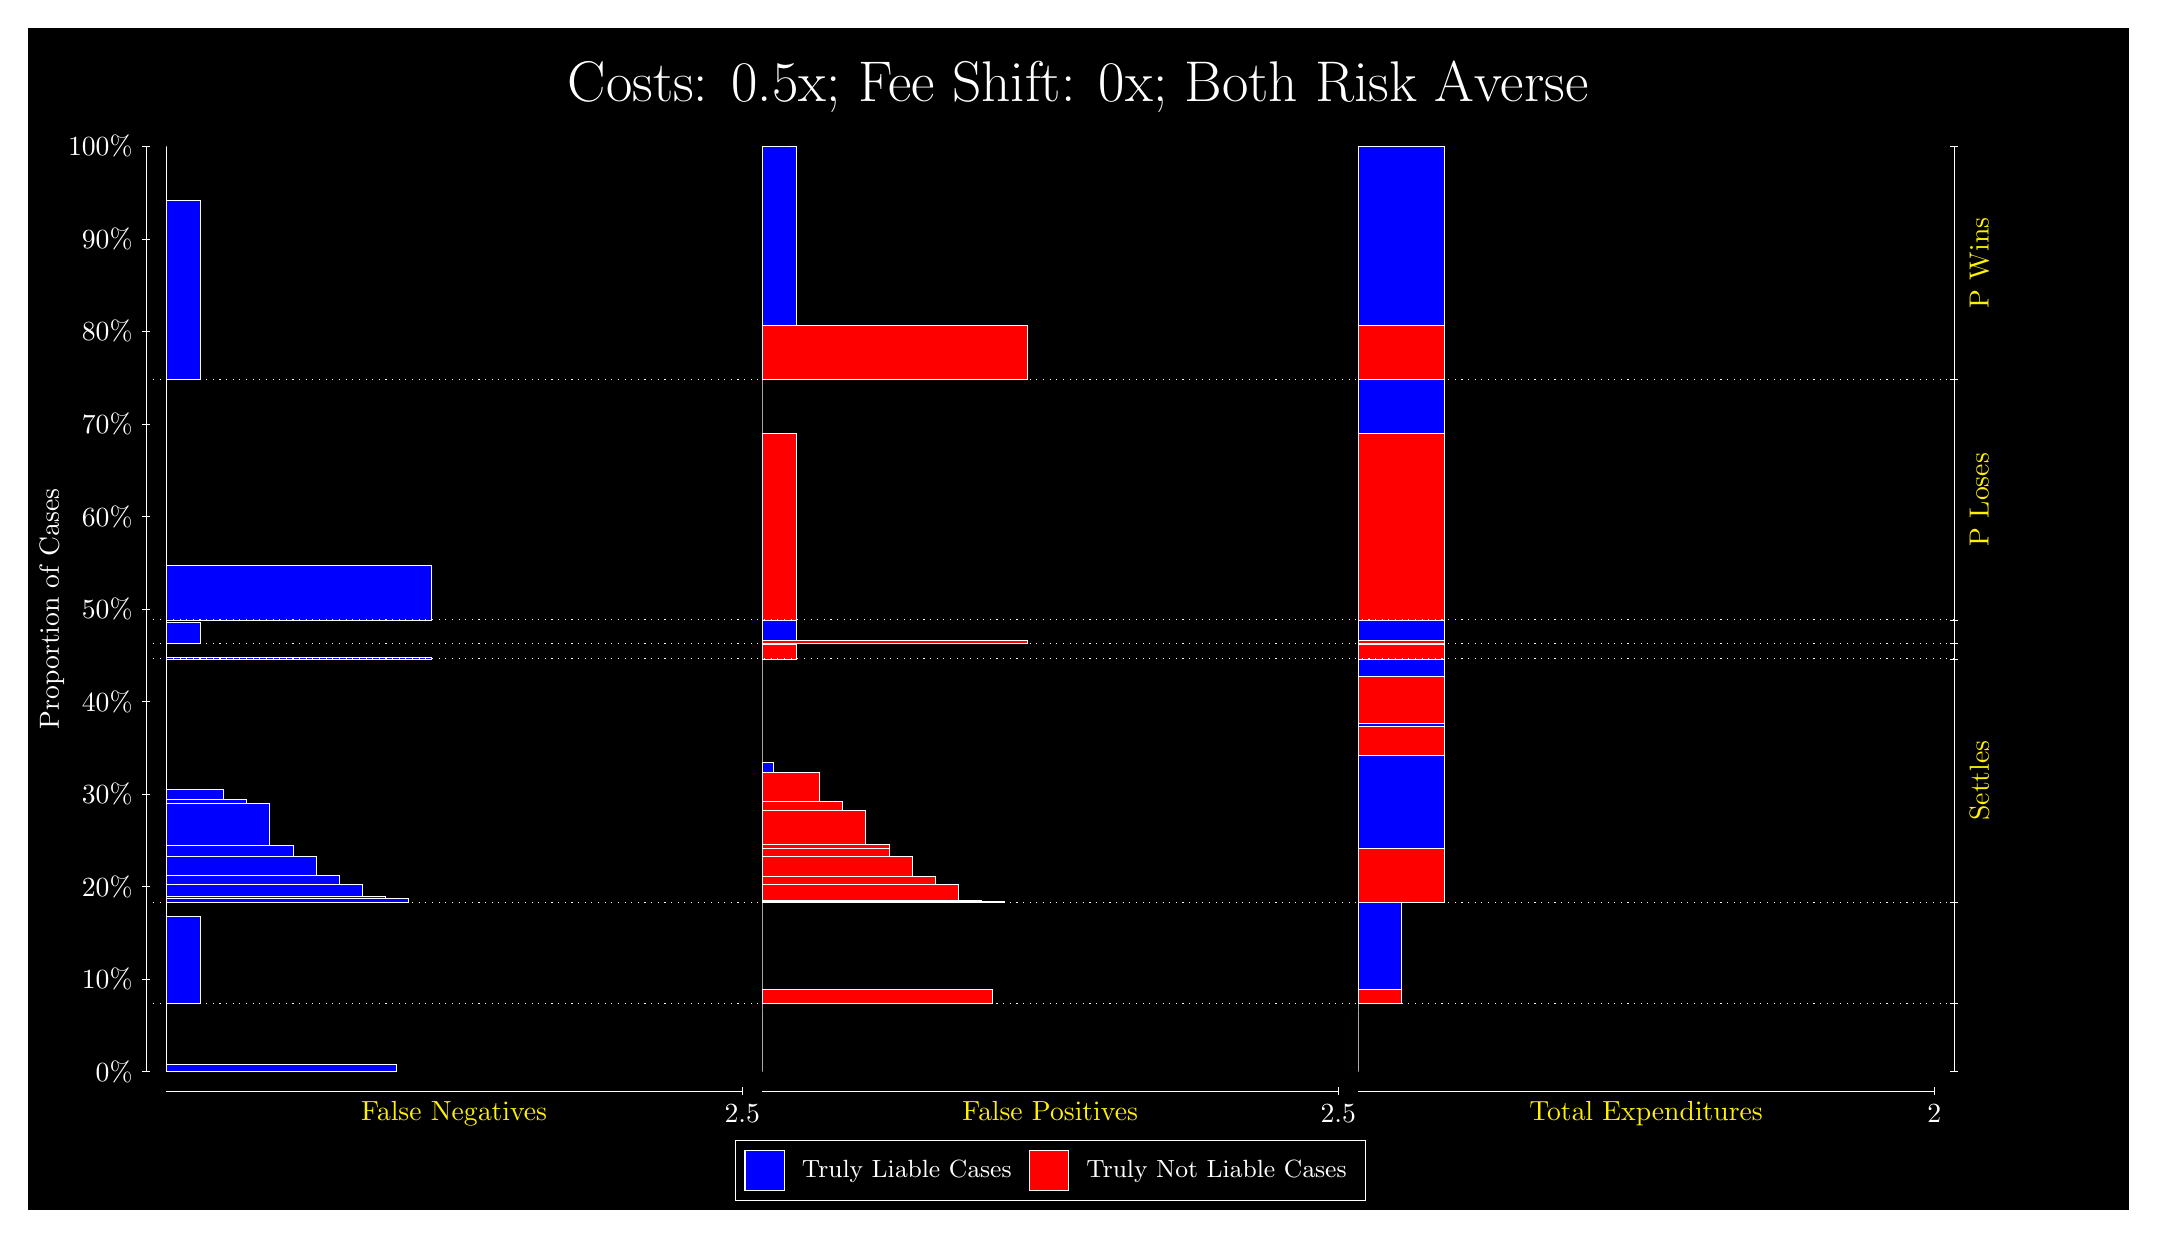
\begin{tikzpicture}
\draw[fill=black] (0,0) rectangle (26.667,15);
\draw[text=white] (0,13.5) rectangle (26.667,15) node[midway] {\huge Costs: 0.5x; Fee Shift: 0x; Both Risk Averse};
\draw[white, very thin] (1.5,1.75) -- (1.5,13.5);
\node[rotate=90, text=white, anchor=center] at (0.3, 7.625) {Proportion of Cases};
\draw[white, very thin] (1.45,1.75) -- (1.55,1.75);
\node[text=white, anchor=east] at (1.45, 1.75) {0\%};
\draw[white, very thin] (1.45,2.925) -- (1.55,2.925);
\node[text=white, anchor=east] at (1.45, 2.925) {10\%};
\draw[white, very thin] (1.45,4.1) -- (1.55,4.1);
\node[text=white, anchor=east] at (1.45, 4.1) {20\%};
\draw[white, very thin] (1.45,5.275) -- (1.55,5.275);
\node[text=white, anchor=east] at (1.45, 5.275) {30\%};
\draw[white, very thin] (1.45,6.45) -- (1.55,6.45);
\node[text=white, anchor=east] at (1.45, 6.45) {40\%};
\draw[white, very thin] (1.45,7.625) -- (1.55,7.625);
\node[text=white, anchor=east] at (1.45, 7.625) {50\%};
\draw[white, very thin] (1.45,8.8) -- (1.55,8.8);
\node[text=white, anchor=east] at (1.45, 8.8) {60\%};
\draw[white, very thin] (1.45,9.975) -- (1.55,9.975);
\node[text=white, anchor=east] at (1.45, 9.975) {70\%};
\draw[white, very thin] (1.45,11.15) -- (1.55,11.15);
\node[text=white, anchor=east] at (1.45, 11.15) {80\%};
\draw[white, very thin] (1.45,12.325) -- (1.55,12.325);
\node[text=white, anchor=east] at (1.45, 12.325) {90\%};
\draw[white, very thin] (1.45,13.5) -- (1.55,13.5);
\node[text=white, anchor=east] at (1.45, 13.5) {100\%};

\draw[white, very thin] (24.457,1.75) -- (24.457,13.5);
\draw[white, very thin] (24.407,1.75) -- (24.507,1.75);
\node[anchor=west] at (24.407, 1.75) {};
\draw[white, very thin] (24.407,2.6135) -- (24.507,2.6135);
\node[anchor=west] at (24.407, 2.6135) {};
\draw[white, very thin] (24.407,3.9003) -- (24.507,3.9003);
\node[anchor=west] at (24.407, 3.9003) {};
\draw[white, very thin] (24.407,6.9901) -- (24.507,6.9901);
\node[anchor=west] at (24.407, 6.9901) {};
\draw[white, very thin] (24.407,7.191) -- (24.507,7.191);
\node[anchor=west] at (24.407, 7.191) {};
\draw[white, very thin] (24.407,7.4868) -- (24.507,7.4868);
\node[anchor=west] at (24.407, 7.4868) {};
\draw[white, very thin] (24.407,10.539) -- (24.507,10.539);
\node[anchor=west] at (24.407, 10.539) {};
\draw[white, very thin] (24.407,13.5) -- (24.507,13.5);
\node[anchor=west] at (24.407, 13.5) {};

\draw[white, very thin, fill=blue] (1.75,1.75) rectangle (4.6775,1.8408);
\draw[white, very thin, fill=red] (1.75,1.8408) rectangle (1.75,2.6135);
\draw[white, very thin, fill=blue] (1.75,2.6135) rectangle (2.1891,3.724);
\draw[white, very thin, fill=red] (1.75,3.724) rectangle (1.75,3.9003);
\draw[white, very thin, fill=blue] (1.75,3.9003) rectangle (4.8239,3.946);
\draw[white, very thin, fill=blue] (1.75,3.946) rectangle (4.5312,3.9733);
\draw[white, very thin, fill=blue] (1.75,3.9733) rectangle (4.2384,4.1335);
\draw[white, very thin, fill=blue] (1.75,4.1335) rectangle (3.9457,4.2367);
\draw[white, very thin, fill=blue] (1.75,4.2367) rectangle (3.6529,4.4781);
\draw[white, very thin, fill=blue] (1.75,4.4781) rectangle (3.3602,4.6199);
\draw[white, very thin, fill=blue] (1.75,4.6199) rectangle (3.0674,5.1608);
\draw[white, very thin, fill=blue] (1.75,5.1608) rectangle (2.7746,5.2132);
\draw[white, very thin, fill=blue] (1.75,5.2132) rectangle (2.4819,5.3349);
\draw[white, very thin, fill=red] (1.75,5.3349) rectangle (1.75,6.9901);
\draw[white, very thin, fill=blue] (1.75,6.9901) rectangle (5.1167,7.0084);
\draw[white, very thin, fill=red] (1.75,7.0084) rectangle (1.75,7.191);
\draw[white, very thin, fill=blue] (1.75,7.191) rectangle (2.1891,7.4506);
\draw[white, very thin, fill=red] (1.75,7.4506) rectangle (1.75,7.4868);
\draw[white, very thin, fill=blue] (1.75,7.4868) rectangle (5.1167,8.1737);
\draw[white, very thin, fill=red] (1.75,8.1737) rectangle (1.75,10.539);
\draw[white, very thin, fill=blue] (1.75,10.539) rectangle (2.1891,12.813);
\draw[white, very thin, fill=red] (1.75,12.813) rectangle (1.75,13.5);
\draw[white, very thin, fill=red] (9.3189,1.75) rectangle (9.3189,2.5227);
\draw[white, very thin, fill=blue] (9.3189,2.5227) rectangle (9.3189,2.6135);
\draw[white, very thin, fill=red] (9.3189,2.6135) rectangle (12.246,2.7898);
\draw[white, very thin, fill=blue] (9.3189,2.7898) rectangle (9.3189,3.9003);
\draw[white, very thin, fill=red] (9.3189,3.9003) rectangle (12.393,3.9132);
\draw[white, very thin, fill=red] (9.3189,3.9132) rectangle (12.1,3.9233);
\draw[white, very thin, fill=red] (9.3189,3.9233) rectangle (11.807,4.1236);
\draw[white, very thin, fill=red] (9.3189,4.1236) rectangle (11.515,4.2298);
\draw[white, very thin, fill=red] (9.3189,4.2298) rectangle (11.222,4.4868);
\draw[white, very thin, fill=red] (9.3189,4.4868) rectangle (10.929,4.5885);
\draw[white, very thin, fill=red] (9.3189,4.5885) rectangle (10.929,4.6391);
\draw[white, very thin, fill=red] (9.3189,4.6391) rectangle (10.636,5.0696);
\draw[white, very thin, fill=red] (9.3189,5.0696) rectangle (10.344,5.1873);
\draw[white, very thin, fill=red] (9.3189,5.1873) rectangle (10.051,5.5555);
\draw[white, very thin, fill=blue] (9.3189,5.5555) rectangle (9.4652,5.6771);
\draw[white, very thin, fill=blue] (9.3189,5.6771) rectangle (9.3189,6.9901);
\draw[white, very thin, fill=red] (9.3189,6.9901) rectangle (9.758,7.1727);
\draw[white, very thin, fill=blue] (9.3189,7.1727) rectangle (9.3189,7.191);
\draw[white, very thin, fill=red] (9.3189,7.191) rectangle (12.686,7.2272);
\draw[white, very thin, fill=blue] (9.3189,7.2272) rectangle (9.758,7.4868);
\draw[white, very thin, fill=red] (9.3189,7.4868) rectangle (9.758,9.8525);
\draw[white, very thin, fill=blue] (9.3189,9.8525) rectangle (9.3189,10.539);
\draw[white, very thin, fill=red] (9.3189,10.539) rectangle (12.686,11.226);
\draw[white, very thin, fill=blue] (9.3189,11.226) rectangle (9.758,13.5);
\draw[white, very thin, fill=red] (16.888,1.75) rectangle (16.888,2.5227);
\draw[white, very thin, fill=blue] (16.888,2.5227) rectangle (16.888,2.6135);
\draw[white, very thin, fill=red] (16.888,2.6135) rectangle (17.437,2.7898);
\draw[white, very thin, fill=blue] (16.888,2.7898) rectangle (17.437,3.9003);
\draw[white, very thin, fill=red] (16.888,3.9003) rectangle (17.986,4.5885);
\draw[white, very thin, fill=blue] (16.888,4.5885) rectangle (17.986,5.7631);
\draw[white, very thin, fill=red] (16.888,5.7631) rectangle (17.986,6.1312);
\draw[white, very thin, fill=blue] (16.888,6.1312) rectangle (17.986,6.1769);
\draw[white, very thin, fill=red] (16.888,6.1769) rectangle (17.986,6.7757);
\draw[white, very thin, fill=blue] (16.888,6.7757) rectangle (17.986,6.9901);
\draw[white, very thin, fill=red] (16.888,6.9901) rectangle (17.986,7.1727);
\draw[white, very thin, fill=blue] (16.888,7.1727) rectangle (17.986,7.191);
\draw[white, very thin, fill=red] (16.888,7.191) rectangle (17.986,7.2272);
\draw[white, very thin, fill=blue] (16.888,7.2272) rectangle (17.986,7.4868);
\draw[white, very thin, fill=red] (16.888,7.4868) rectangle (17.986,9.8525);
\draw[white, very thin, fill=blue] (16.888,9.8525) rectangle (17.986,10.539);
\draw[white, very thin, fill=red] (16.888,10.539) rectangle (17.986,11.226);
\draw[white, very thin, fill=blue] (16.888,11.226) rectangle (17.986,13.5);
\draw[white, dotted] (1.5,2.6135) -- (24.457,2.6135);
\draw[white, dotted] (1.5,3.9003) -- (24.457,3.9003);
\draw[white, dotted] (1.5,6.9901) -- (24.457,6.9901);
\draw[white, dotted] (1.5,7.191) -- (24.457,7.191);
\draw[white, dotted] (1.5,7.4868) -- (24.457,7.4868);
\draw[white, dotted] (1.5,10.539) -- (24.457,10.539);
\draw[white, very thin] (1.75,1.5) -- (9.0689,1.5);
\node[text=yellow, anchor=north] at (5.4094, 1.5) {False Negatives};
\draw[white, very thin] (9.0689,1.45) -- (9.0689,1.55);
\node[text=white, anchor=north] at (9.0689, 1.45) {2.5};

\draw[white, very thin] (9.3189,1.5) -- (16.638,1.5);
\node[text=yellow, anchor=north] at (12.978, 1.5) {False Positives};
\draw[white, very thin] (16.638,1.45) -- (16.638,1.55);
\node[text=white, anchor=north] at (16.638, 1.45) {2.5};

\draw[white, very thin] (16.888,1.5) -- (24.207,1.5);
\node[text=yellow, anchor=north] at (20.547, 1.5) {Total Expenditures};
\draw[white, very thin] (24.207,1.45) -- (24.207,1.55);
\node[text=white, anchor=north] at (24.207, 1.45) {2};



\node[text=yellow, centered, rotate=90] at (24.777, 5.4452) {Settles};


\node[text=yellow, centered, rotate=90] at (24.777, 9.0131) {P Loses};
\node[text=yellow, centered, rotate=90] at (24.777, 12.02) {P Wins};

\draw (12.978300999999998,1.5) node[draw=none] (baseCoordinate) {};
\begin{scope}[align=center]
        \matrix[scale=0.5, draw=white, below=0.5cm of baseCoordinate, nodes={draw}, column sep=0.1cm]{
            \node[rectangle, draw, minimum width=0.5cm, minimum height=0.5cm, fill=blue] {}; &
            \node[draw=none, font=\small, text=white] (B) {Truly Liable Cases}; &
            \node[rectangle, draw, minimum width=0.5cm, minimum height=0.5cm, fill=red] {}; &
            \node[draw=none, font=\small, text=white] (B) {Truly Not Liable Cases}; \\
            };
\end{scope}

\end{tikzpicture}
\end{document}